\documentclass[serif, xcolor=dvipsnames]{beamer}

\makeatletter

% HAY QUE ELEGIR EL QUE CORRESPONDA

%\usepackage{mathpazo}%Letra palatino con fuentes para matemáticas
\usepackage[T1]{fontenc}
\usepackage[utf8]{inputenc}
\usepackage{graphicx}
\usepackage{url}
\usepackage{amsmath}
\usepackage{booktabs}
\usepackage{textcomp}%%needed for the euro symbol

\date{}

\usepackage[emulate=units]{siunitx}
\sisetup{per=fraction, fraction=nice, decimalsymbol=comma}
\newunit{\wattpeak}{Wp}
\newunit{\watthour}{Wh}
\newunit{\amperehour}{Ah}

\setbeamercovered{transparent}
\setbeamertemplate{navigation symbols}{}
\usefonttheme{structuresmallcapsserif} 
\usefonttheme{serif} 
\usefonttheme{structurebold}

%\usepackage{epstopdf}


\usepackage[spanish]{babel}
\addto\shorthandsspanish{\spanishdeactivate{~<>}}

\hypersetup{pdfauthor={Oscar Perpi\~n\'an},%
    pdftitle={Energ\'ia Solar Fotovoltaica},%
    filecolor=blue,%
    urlcolor=blue}



%\usepackage{handoutWithNotes} %para hacer papel con notas 
%\pgfpagesuselayout{4 on 1 with notes}[a4paper,border shrink=5mm]



%\usepackage{pgfpages}
%\pgfpagesuselayout{2 on 1}[a4paper,border shrink=5mm]

 
%\usepackage{mathpazo}%Letra palatino con fuentes para matemáticas
\usepackage[T1]{fontenc}
\usepackage[utf8]{inputenc}
\usepackage{graphicx}
\usepackage{url}
\usepackage{amsmath}
\usepackage{booktabs}

\usepackage[spanish]{babel}
\addto\shorthandsspanish{\spanishdeactivate{~<>}}


\usepackage{hyperref}
% \hypersetup{pdfauthor={Oscar Perpi\~n\'an},%
%     pdftitle={Energ\'ia Solar Fotovoltaica},%
%     filecolor=blue,%
%     urlcolor=blue}

\hypersetup{
    bookmarks=true,         % show bookmarks bar?
%    unicode=true,          % non-Latin characters in Acrobat’s bookmarks
    bookmarksnumbered=false,
    bookmarksopen=false,
    breaklinks=true,
    backref=true,
    pdftoolbar=true,        % show Acrobat’s toolbar?
    pdfmenubar=true,        % show Acrobat’s menu?
    pdffitwindow=false,     % window fit to page when opened
    pdfstartview={FitH},    % fits the width of the page to the window
    pdftitle={Energía Solar Fotovoltaica},    % title
    pdfauthor={Oscar Perpiñán Lamigueiro},     % author
    pdfsubject={Electrotecnia},   % subject of the document
    pdfcreator={AucTeX/Emacs},   % creator of the document
    pdfproducer={LaTeX}, % producer of the document
    pdfnewwindow=true,      % links in new window
    pdfborder={0 0 0},
    colorlinks=true,       % false: boxed links; true: colored links
    linkcolor=,          % color of internal links
    citecolor=BrickRed,        % color of links to bibliography
    filecolor=black,      % color of file links
    urlcolor=Blue           % color of external links 
}

\usepackage[emulate=units]{siunitx}
\sisetup{per=fraction, fraction=nice, decimalsymbol=comma}
\newunit{\wattpeak}{Wp}
\newunit{\watthour}{Wh}
\newunit{\amperehour}{Ah}

\setbeamercovered{transparent}
\setbeamertemplate{navigation symbols}{}
\usefonttheme{serif} 
\usefonttheme{structuresmallcapsserif} 

\useinnertheme[shadow=true]{rounded}
\useoutertheme{shadow}
%\usecolortheme[named=BrickRed]{structure} %sirve para cambiar el color genérico
\usecolortheme{orchid}
\usecolortheme{whale}
\documentclass[xcolor={usenames,svgnames,dvipsnames}]{beamer}
\usepackage[utf8]{inputenc}
\usepackage[T1]{fontenc}
\usepackage{graphicx}
\usepackage{grffile}
\usepackage{longtable}
\usepackage{wrapfig}
\usepackage{rotating}
\usepackage[normalem]{ulem}
\usepackage{amsmath}
\usepackage{textcomp}
\usepackage{amssymb}
\usepackage{capt-of}
\usepackage{hyperref}
\usepackage{color}
\usepackage{listings}
\usepackage{mathpazo}
\usepackage{gensymb}
\usepackage{amsmath}
\usepackage{chemarr}%flechas para reacciones químicas (SFER.tex)
\bibliographystyle{plain}
\AtBeginSubsection[]{\begin{frame}[plain]\tableofcontents[currentsubsection,sectionstyle=show/shaded,subsectionstyle=show/shaded/hide]\end{frame}}
\AtBeginSection[]{\begin{frame}[plain]\tableofcontents[currentsection,hideallsubsections]\end{frame}}
\usepackage[emulate=units]{siunitx}
\sisetup{fraction=nice, decimalsymbol=comma, retain-unity-mantissa = false}
\newunit{\wattpeak}{Wp}
\newunit{\watthour}{Wh}
\newunit{\amperehour}{Ah}
\usepackage{steinmetz}
\hypersetup{colorlinks=true, linkcolor=OliveGreen, urlcolor=Blue}
\renewcommand{\thefootnote}{\fnsymbol{footnote}}
\beamertemplatenavigationsymbolsempty
\setbeamertemplate{footline}[frame number]

\setbeamercolor{alerted text}{fg=Green!50!black} \setbeamerfont{alerted text}{series=\bfseries}
\usefonttheme{serif}
\setbeamercovered{transparent}
\setbeamertemplate{navigation symbols}{}
\usefonttheme{serif} 

\setbeamercolor{palette primary}{bg=OliveGreen,fg=white}
\setbeamercolor{palette secondary}{bg=OliveGreen,fg=white}
\setbeamercolor{palette tertiary}{bg=OliveGreen,fg=white}
\setbeamercolor{palette quaternary}{bg=OliveGreen,fg=white}
\setbeamercolor{structure}{fg=OliveGreen} % itemize, enumerate, etc
\setbeamercolor{section in toc}{fg=OliveGreen} % TOC sections

\usetheme[hideothersubsections]{Goettingen}

\usepackage{tikz}

\titlegraphic{
\includegraphics[width=2.5cm]{../figs/logoEOI.jpg}}
\addtobeamertemplate{frametitle}{}{%
\begin{tikzpicture}[remember picture,overlay]
\node[anchor=south east,yshift=2pt] at (current page.south east) {
\includegraphics[width=1.5cm]{../figs/logoEOI.jpg}};
\end{tikzpicture}}


\makeatother

\usepackage[spanish]{babel}
\addto\shorthandsspanish{\spanishdeactivate{~<>}}

\begin{document}

\title[\textsc{SFCR: Diseño}]{\textsc{Sistemas Fotovoltaicos }\\
  \textsc{de Conexión a Red}}

\subtitle{Diseño}


\author{\textsc{Oscar Perpiñán Lamigueiro}} \date{}

\frame[plain]{\titlepage}

\AtBeginSection[]{
  \begin{frame}[plain]
    \frametitle{Índice}
    % \setcounter{tocdepth}{1}
    \tableofcontents[currentsection]
  \end{frame}

}

\selectlanguage{spanish}%

\section{Generador Fotovoltaico}


\begin{frame}[plain]
  \frametitle{Inclinación y Orientacion}

\[
\beta_{opt}=3.7+0.69 \cdot \left|\phi\right|\]


\begin{center}
  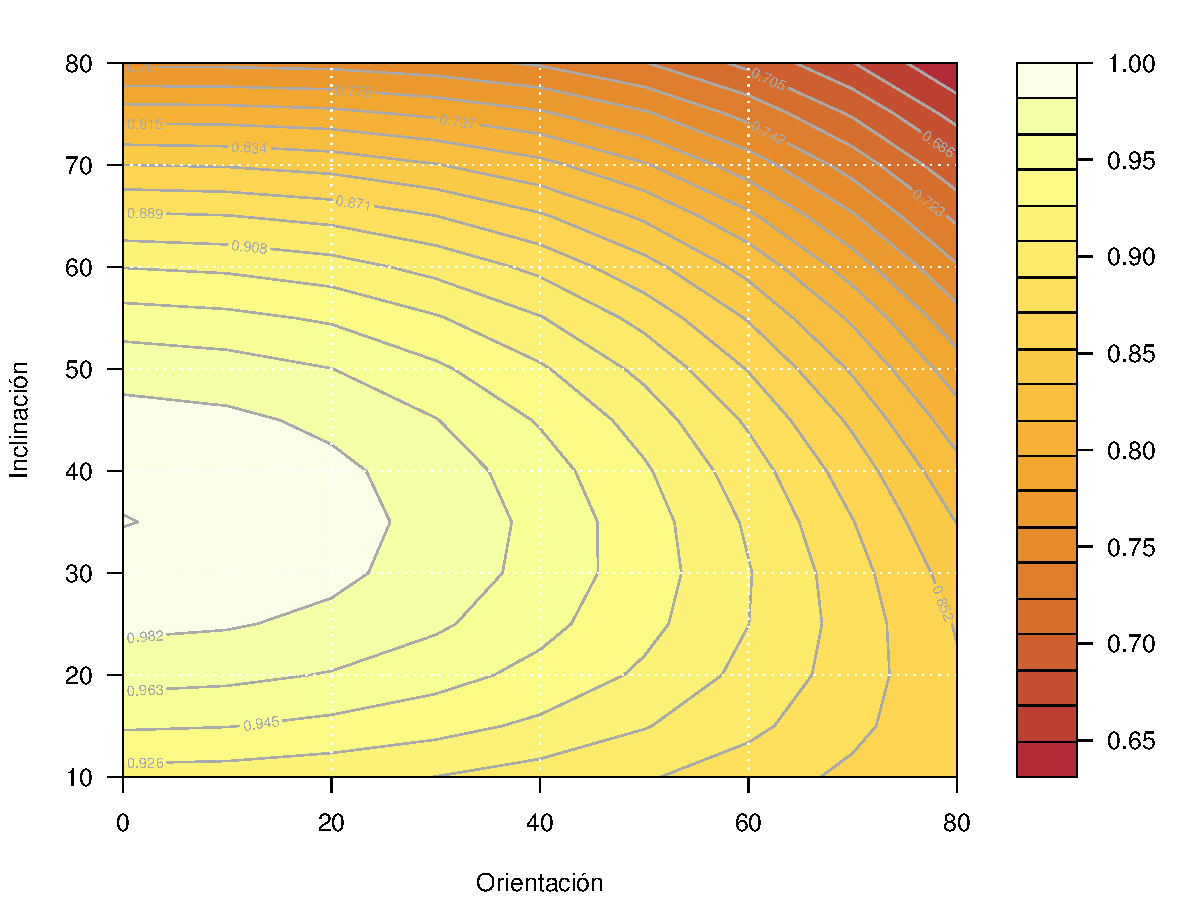
\includegraphics[scale=0.5]{../Figuras/PorcentajeProduccionEdificios}
  \par\end{center}


\end{frame}

\begin{frame}
  \frametitle{Pérdidas angulares según CTE}

\[
\mathrm{
  \begin{cases}
    100\cdot[1,2\cdot10^{-4}\cdot(\beta-\phi+10)^{2}+3,5\cdot10^{-5}\cdot\alpha^{2}]
    & 15\degree<\beta<90\degree\\
    100\cdot[1,2\cdot10^{-4}\cdot(\beta-\phi+10)^{2}] &
    \beta<15\degree
  \end{cases}}
\]


\begin{center}
  \begin{tabular}{>{\centering}m{3cm}>{\centering}m{3cm}cc}
    \toprule 
    \textrm{Caso} & \textrm{Orientación e inclinación} & \textrm{Sombras} & \textrm{Total}\tabularnewline
    \midrule
    \midrule 
    \textrm{General } & \textrm{10} & \textrm{10} & \textrm{15}\tabularnewline
    \midrule 
    \textrm{Superposición} & \textrm{20} & \textrm{15} & 30\tabularnewline
    \midrule 
    \textrm{Integración arquitectónica} & 40 & 20 & 50\tabularnewline
    \bottomrule
  \end{tabular}
  \par\end{center}


\end{frame}
\begin{frame}
  \frametitle{Modulos en serie}
  \begin{itemize}
  \item El inversor está diseñado para soportar una \textbf{tensión
      máxima en la entrada}. Superarla puede conllevar la avería del
    equipo.
  \item Por otra parte, el algoritmo de \textbf{búsqueda del MPP} se
    realiza en un rango de tensiones limitado. Para evitar pérdidas
    por trabajar en un punto alejado del MPP, la tensión del generador
    debe estar dentro de este rango.\end{itemize}
  \begin{block} {}

\[
N_{s,max}:\, V_{ocG}(G=\SI{200}{\watt\per\meter\squared},\,
T_{a}=\SI{-10}{\celsius})<V_{max,inv}\]
\[
N_{s,mpp}:\, V_{mppG}(G_{stc},\,
T_{a}=\SI{25}{\celsius})\in\left[V_{mppMIN},\,
  V_{mppMAX}\right]_{INV}\]


\end{block}

\end{frame}
\begin{frame}
  \frametitle{Ramas en paralelo}

  El fabricante del inversor elige los componentes para soportar una
  \textbf{corriente máxima admisible}.

  En general, el inversor es capaz de autoprotegerse ante valores
  superiores a este umbral desplazando el punto de funcionamiento del
  generador fuera del MPP.

  No obstante, el diseñador del sistema debe elegir el número de ramas
  en paralelo de forma que no se supere este umbral.
  \begin{block} {}

\[
N_{p,max}:\, I_{scG}(\SI{1000}{\watt\per\meter\squared})<I_{max,INV}\]


\end{block}

\end{frame}
\begin{frame}
  \frametitle{Configuración del generador}

  De los cálculos anteriores se obtiene una ventana de configuraciones
  del generador que permiten un buen acoplamiento entre inversor y
  generador.  Para elegir una configuración deben tenerse en cuenta
  diferentes aspectos:
  \begin{itemize}
  \item Configuración eléctrica y ubicación física de los módulos en
    la estructura.
  \item La curva de eficiencia del inversor depende de la tensión de
    entrada.
  \item Inversión y rendimiento económicos.
  \item Espacio disponible.
  \item Relación de potencias de generador e inversor.
  \end{itemize}

\end{frame}
\begin{frame}
  \frametitle{Configuración eléctrica y estructura}
  \begin{itemize}
  \item Es recomendable elegir \textbf{series} compuestas por un
    número de módulos que puedan ser ubicados en una \textbf{única
      hilera de la estructura}.

    \begin{itemize}
    \item \textbf{Se facilita el trazado del cableado}: la propia
      estructura puede servir como fijación auxiliar, se evitan
      cruzamientos indeseados.
    \item \textbf{Se minimiza la influencia de las sombras}: es muy
      frecuente la aparición de sombras entre partes del generador o
      entre seguidores, sombras de forma rectangular y que comienzan
      afectando a las partes bajas de la estructura. Al cablear por
      hileras, las sombras de las hileras bajas no afectan a las
      hileras inmediatamente superiores.
    \end{itemize}
  \end{itemize}

\end{frame}
\begin{frame}
  \frametitle{Potencia del generador}
  \begin{itemize}
  \item La potencia del generador fotovoltaico está relacionada
    directamente con la \textbf{inversión económica} a realizar.
  \item Por otra parte, la relación entre \textbf{energía generada} y
    potencia nominal es aproximadamente lineal, y por tanto, los
    \textbf{ingresos económicos} dependen casi linealmente de la
    potencia del generador.
  \item Por tanto, para decidir la potencia del generador
    ($P_{g}^{*}=N_{s}\cdot N_{p}\cdot P_{m}^{*}$) debe tenerse en
    cuenta el capital o financiación disponible, y el rendimiento
    económico deseado.
  \end{itemize}

\end{frame}
\begin{frame}
  \frametitle{Potencia del generador}
  \begin{itemize}
  \item La potencia del generador es proporcional al área del
    generador y al \textbf{terreno ocupado }(que también influye,
    aunque en menor grado, en el cálculo económico). Por tanto, debe
    tenerse en cuenta el espacio disponible (o el coste que se
    pretende asumir por el uso de terreno).
  \item Según el \textbf{tipo de sistema} (estático, seguimiento) se
    debe elegir una relación de potencias de generador e inversor.
  \end{itemize}

\end{frame}


\section{Inversor}


\begin{frame}
  \frametitle{Curva de eficiencia}

  Para calcular la potencia entregada por el inversor a partir de la
  potencia suministrada por el generador fotovoltaico se empleará la
  curva de eficiencia del inversor, $\eta_{inv}$, definida como la
  relación entre la potencia suministrada a la red eléctrica,
  $P_{ac}$, y la potencia de entrada, $P_{dc}$. Esta relación puede
  describirse con una función basada en tres coeficientes y la
  normalización de la potencia de salida:

\[
\eta_{inv}=\frac{p_{o}}{p_{o}+k_{0}^{o}+k_{1}^{o}p_{o}+k_{2}^{o}p_{o}^{2}}\]
donde $p_{o}=P_{ac}/P_{inv}$, y $k_{0}^{o}$, $k_{1}^{o}$ y $k_{2}^{o}$
son parámetros adimensionales que definen el comportamiento eléctrico
del inversor.


\end{frame}
\begin{frame}
  \frametitle{Curva de eficiencia}
  \begin{columns}[c]%{}


    \column{3cm}

    $k_{0}^{o}=0.01$

    $k_{1}^{o}=0.025$

    $k_{2}^{o}=0.05$


    \column{7cm}

    \begin{center}
      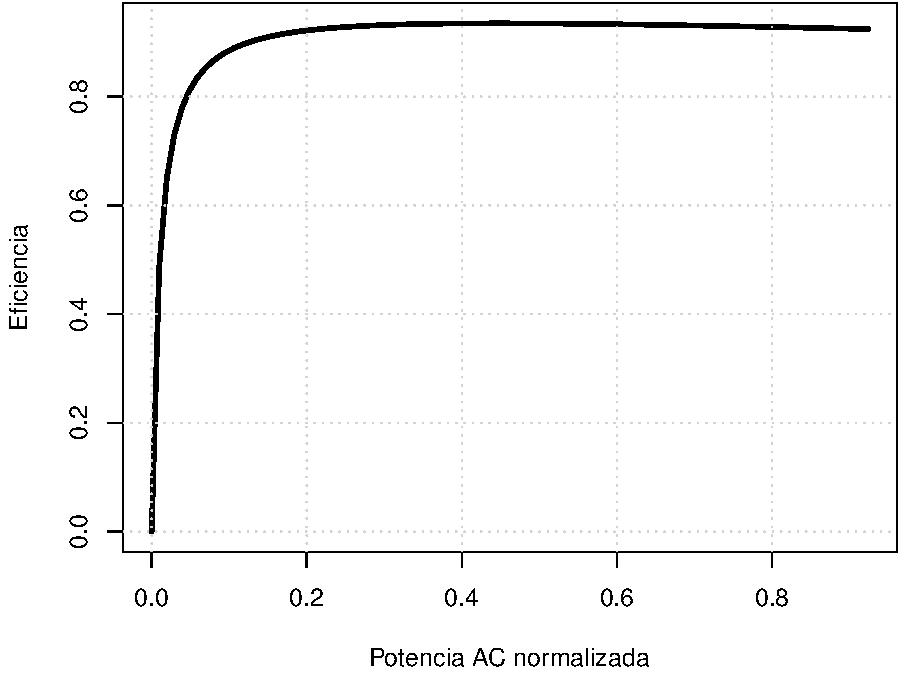
\includegraphics[scale=0.5]{../Figuras/CurvaInversor}
      \par\end{center}

  \end{columns}%{}

\end{frame}
\begin{frame}
  \frametitle{Relación de potencias}
  \begin{itemize}
  \item Dado que la potencia entregada por el generador varía con las
    condiciones meteorológicas, el inversor trabajará en diferentes
    zonas de su curva de eficiencia.
  \item Por tanto, una de las preguntas a responder es qué relación
    debe existir entre la potencia del generador FV y el inversor.
  \item Si esta relación es alta, el inversor trabajará con frecuencia
    en la región de alta eficiencia, pero a cambio es posible que deba
    limitar la potencia del generador para evitar superar su umbral de
    corriente admisible.
  \end{itemize}

\end{frame}
\begin{frame}
  \frametitle{Relación de potencias}
  \begin{itemize}
  \item En \textbf{sistemas de integración arquitectónica}, donde la
    orientación e inclinación no son óptimas, esta probabilidad puede
    ser baja. Así, puede considerarse necesario sobredimensionar el
    generador FV respecto al inversor
    ($P_{g}^{*}/P_{inv}\in\left[1;1.4\right]$).

    \begin{itemize}
    \item CTE-HE5-3.2.3.2: {}``la potencia del inversor será como
      mínimo el 80\% de la potencia pico real del generador
      fotovoltaico''
    \end{itemize}
  \item En \textbf{sistemas de seguimiento} esta probabilidad suele
    ser alta.  Se recomiendan inversores de potencia similar a la del
    generador ($P_{g}^{*}/P_{inv}\in\left[1;1.2\right]$)
  \end{itemize}

\end{frame}
\begin{frame}
  \frametitle{Relación de potencias}
  \begin{block} {}

    No obstante, es posible demostrar que el valor de esta relación no
    es tan crítico como \textbf{elegir un inversor con buena curva de
      eficiencia}.

  \end{block}
\end{frame}

\section{Cableado}


\begin{frame}
  \frametitle{Características básicas}
  \begin{columns}[c]%{}


    \column{6cm}
    \begin{itemize}
    \item Diseño del cableado

      \begin{itemize}
      \item Criterio de caída de tensión
      \item En sistemas de gran tamaño reducir bucles
      \item Diseño de estructura e integración: habilitar un camino
        para cableado
      \end{itemize}
    \item Tipo de cables

      \begin{itemize}
      \item Doble aislamiento
      \item Poliolefínas
      \end{itemize}
    \end{itemize}

    \column{6cm}

    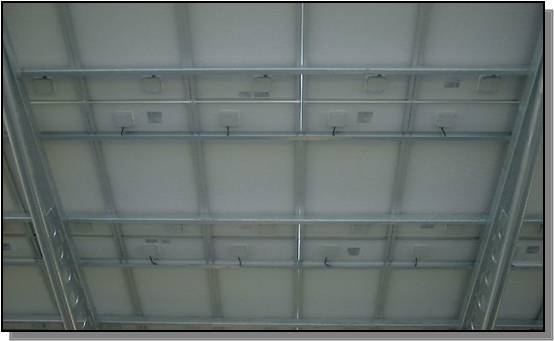
\includegraphics[scale=0.6]{../Fotos/PhotocampaCableado}

  \end{columns}%{}

\end{frame}
\begin{frame}
  \frametitle{Cálculo}

  Habitualmente se descarta el criterio termico y se emplea el
  criterio de caida de tensión (RBT ITC-BT-07):\begin{eqnarray*}
    S_{dc} & = & \frac{2\cdot L_{dc}\cdot I_{dc}}{56\cdot\Delta V_{dc}}\\
    S_{1ac} & = & \frac{2\cdot L_{1ac}\cdot I_{1ac}}{56\cdot\Delta V_{1ac}}\\
    S_{3ac} & = & \frac{\sqrt{3}\cdot L_{3ac}\cdot
      I_{3ac}}{56\cdot\Delta V_{3ac}}\end{eqnarray*}


  En general, se suele aceptar una caída máxima de tensión
  $\SI{1.5}{\percent}$ de la tensión nominal. Para aplicar
  correctamente este porcentaje es importante caer en la cuenta de que
  cada zona (DC y AC) tiene su propia tensión nominal.


\end{frame}
\begin{frame}
  \frametitle{Cálculo}
  \begin{block} {Ejemplo}

    Por ejemplo, en una instalación que conduce $\SI{75}{\ampere}$ a
    la salida de un inversor trifásico, situado este a
    $\SI{100}{\meter}$ de la conexión a red, se deberá utilizar un
    cable de sección
    $S=\frac{\sqrt{3}\cdot100\cdot75}{56\cdot\SI{1.5}{\percent}\cdot400}=\SI{38.66}{\milli\meter\squared}$.

    Dado que la sección de los cables está normalizada, se deberá
    optar por la sección inmediatamente superior, y por tanto la
    conexión del inversor a la red se realizará con tres cables de
    sección $S=\SI{50}{\milli\meter\squared}$.

  \end{block}

\end{frame}
\begin{frame}
  \frametitle{Cálculo}
  \begin{block} {}

    Con este resultado, es necesario comprobar que la intensidad de
    diseño es inferior a la intensidad máxima admisible del cable para
    sus condiciones de servicio, según las tablas de la ITC-BT-07.

    No obstante, las secciones que resultan del criterio de caída de
    tensión aplicado a los sistemas fotovoltaicos habitualmente son
    sobradamente capaces de conducir la corriente del sistema.

  \end{block}

\end{frame}
\begin{frame}
  \frametitle{Cálculo}

  Suponiendo que en una planta con varios inversores trifásicos existe
  la posibilidad de ubicar los inversores debajo del generador FV
  (\emph{distribución en alterna}) o en un centro específico junto al
  punto de conexión a red (\emph{distribución en continua}),
  \textbf{¿cuál es la tensión de trabajo en continua que permite optar
    por una distribución en continua?}


\end{frame}

\end{document}
